\documentclass[11pt]{article}

% Scientific-journal working set — all served ONLY by the `academic` tier, so the
% §5.4(a) static \usepackage scan must preselect + mount `academic` before pass 1.
\usepackage{siunitx}     % academic (collection-mathscience)
\usepackage{mathtools}   % academic (collection-mathscience)
\usepackage{pgfplots}    % academic (collection-pictures); pulls in tikz/pgf
\pgfplotsset{compat=1.16}

% Author-year citation stack. natbib + the plainnat .bst both ship in `core`, so
% the citation pipeline (engine -> bibtex8 -> engine -> engine) resolves from the
% preloaded tier; academic is driven by the math/figure packages above.
\usepackage{natbib}

\title{Thermal Relaxation in Layered Metamaterials}
\author{WasmTeX Conformance Suite}
\date{}

\begin{document}
\maketitle

We measured a relaxation time of \qty{4.2}{\micro\second} under an applied field
of \qty{9.8}{\tesla}, in agreement with the layered-transport model of
\citet{zhang2019}. Comparable dispersion was reported in earlier lattice surveys
\citep{nakamura2021}.

The governing relation for the thermal relaxation time is
\begin{equation}
  \tau \coloneqq \tau_0 \exp\!\left(\frac{E_a}{k_B T}\right),
\end{equation}
where $E_a$ denotes the activation energy and $k_B$ the Boltzmann constant.

\begin{figure}[h]
\centering
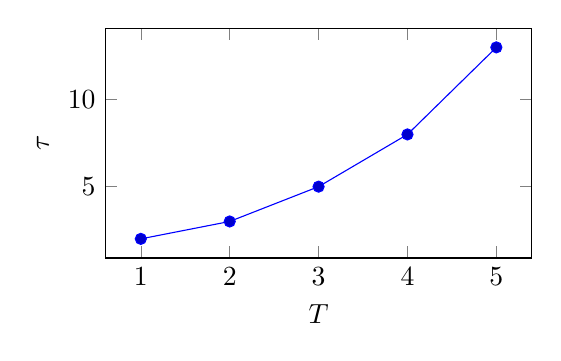
\begin{tikzpicture}
\begin{axis}[width=7cm,height=4.5cm,xlabel={$T$},ylabel={$\tau$}]
\addplot coordinates {(1,2) (2,3) (3,5) (4,8) (5,13)};
\end{axis}
\end{tikzpicture}
\caption{Measured relaxation versus temperature.}
\end{figure}

\bibliographystyle{plainnat}
\bibliography{refs}
\end{document}
